\documentclass{article}
\usepackage[margin=1in]{geometry}
\usepackage{amsmath,amssymb,mathtools}
\usepackage{enumerate}
\usepackage{tikz,tkz-euclide}
\usepackage{float}

\title{Geometry Problem 2}
\author{Andrew McGregor}
\date{}
\begin{document}
\maketitle
\section*{Problem}
Let $ABC$ be a triangle with circumcentre $O$. Let $D$ be the point of intersection between the bisector of $\angle ABC$ and the perpendicular bisector of $AB$. Let the circumcircle of $ADO$ be $\omega$. Let $E\neq A$ be the intersection of $\omega$ with the segment $AB$. Let $P\neq E$ be the intersection of the circumcircle of $COE$ with the line $AB$. Prove that $BQ$ is tangent to $\omega$.
\section*{Solution}

\begin{figure}[H]
	\centering
	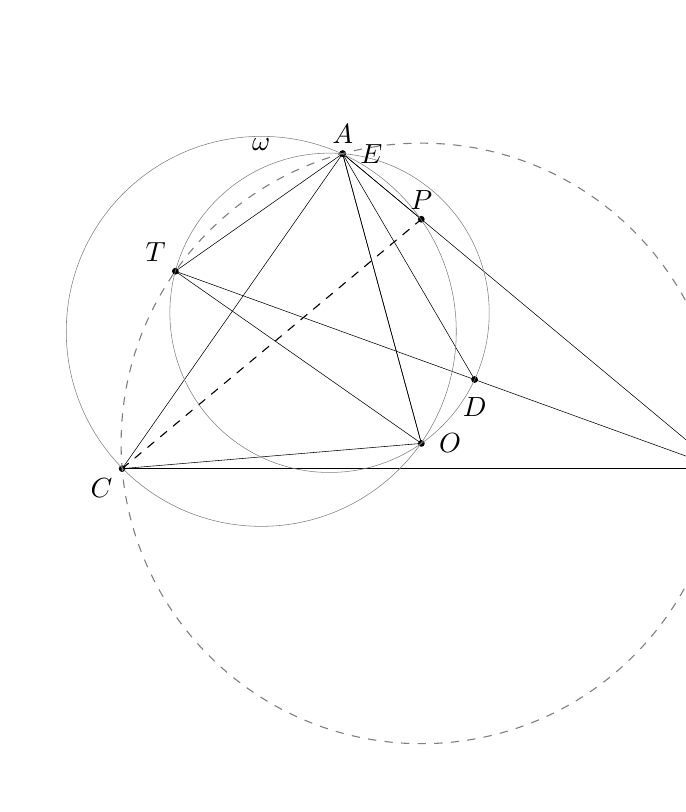
\begin{tikzpicture}[scale=4]
		\useasboundingbox (-1,-1) rectangle (1,1.4);
		\tkzDefPoints{0/1/A, 1.2/0/B, -0.7/0/C}
		\tkzDefCircle[circum](A,B,C)\tkzGetPoint{O}
		\tkzDefLine[bisector](A,B,C)\tkzGetPoint{b1}
		\tkzDefLine[mediator](A,B)\tkzGetPoints{m1}{m2}
		\tkzInterLL(B,b1)(m1,m2)\tkzGetPoint{D}
		\tkzDefCircle[circum](A,D,O)\tkzGetPoint{X}
		\tkzInterLC(A,B)(X,A)\tkzGetSecondPoint{E}
		\tkzDefCircle[circum](C,O,E)\tkzGetPoint{Y}
		\tkzInterCC(O,A)(X,A)\tkzGetFirstPoint{T}
		\tkzInterLC(A,B)(Y,C)\tkzGetFirstPoint{P}
		\tkzDrawPoints[fill=black](A,B,C,D,E,O,T,P)
		\tkzDrawSegments(A,B B,C C,A O,C O,T O,A O,E B,T D,A A,P A,T)
		\tkzDrawSegments[dashed,thin](C,P)
		\tkzDrawCircle(X,A)
		\tkzDrawCircle(Y,C)
		\tkzDrawCircle[dashed,thin](O,A)
		\tkzLabelPoints[below=0.1](D)
		\tkzLabelPoints[right=0.1](O,E)
		\tkzLabelPoints[above](A,P)
		\tkzLabelPoints[above left](T)
		\tkzLabelPoints[below left](B,C)
		\tkzLabelCircle[above=0.1](X,A)(30){$\omega$}

	\end{tikzpicture}
\end{figure}
Let $T$ be the midpoint of the arc $AC$ not containing $B$. We will show that $T$ lies on $\omega$. Note:
\begin{flalign}
	\angle ADT&= \angle ABD + \angle DAB= 2\angle ABD=2\angle ABT=\angle AOT \nonumber
\end{flalign}
 Therefore $T$ lies on $\omega$. Also note that since $\triangle OCT \equiv \triangle OAT$:
\begin{flalign}
 	\angle CTO &= \angle TCO = \angle TAO \nonumber
\end{flalign}
So $CT$ is tangent to $\omega$. Let $P'= CT\cap AB$. We will show that $P' \equiv P$. Note that it is sufficient to show that $P'COE$ is a cyclic quad as this would require $P' \equiv P$. But note that:
\begin{flalign}
 	\angle OEB= \angle OTA =\angle OAT=\angle OCT=\angle OCP
\end{flalign}
So $P'COE$ is a cyclic quad, and so $P' \equiv P$ and thus $CP$ is tangent to $\omega$ at $T$.

\end{document}
